\chapter{Requirements for Supporting Intention-oriented Organizational Modeling}
\label{chap:analysis}
This chapter positions the thesis work in the field of organizational modeling with respect to the other existing approaches. The first section provides detailed requirement analysis of intention-oriented organizational modeling. The last section provides a detailed literature review about the existing approaches. A detailed evaluation of the existing approaches with the proposed requirements is also provided in the last section.

%%%%%%%%%%%%%%%%%%%%%%%%%%%%%%%%%%%%%%%%%%%%%%%%%%%%%%%%%%%%%%%%%%%%%%%%%
\section{Requirement Analysis of Intention-oriented Organizational Modeling}
\label{sec:requirementssupoorting}
%%%%%%%%%%%%%%%%%%%%%%%%%%%%%%%%%%%%%%%%%%%%%%%%%%%%%%%%%%%%%%%%%%%%%%%%%
The requirements of intention-oriented organizational modeling has been derived from existing literatures \cite{McManus2007, Mandic2010,Bleistein2006, Lacom, Brambilla2012} and from the motivating scenario described in Chapter \ref{chap:motivatingScenario}. 

\subsection{Organizational Intention Transparency (R1)}
An intention can be broken down into definitive actionable components upon which individual resources can act. When these lower level intentions are made achievable for individual resources, they can be combined to provide successful execution of higher level intention, i.e., main intention. This requires privilege for different organizational members to observe lower level and higher level intentions. Additionally, intentions should also be traceable from different levels of the organizational hierarchy. This means that the status of each intention can be accessed by members in different levels of the organizations. This level of transparency within an organization reduces inefficiencies during intention execution, and is a key factor in attracting and retaining high performers in the labor market \cite{McManus2007}. Requirement R1 has to be satisfied in the modeling phase itself as the designing of intentions, strategies and their recursive structures are done during the modeling phase. The main pre-requisites for this requirement to be satisfied are, intentions can be refinable and organizational members can view intentions at different levels. 

\subsection{Organizational Strategy-based Cost Estimation (R2)}
Linking strategies with capabilities that has matching resource enable us a cost estimation for each strategy. This is because strategies are associated with organizational capabilities which in turn are associated with organizational resources. To incorporate the cost estimation of strategies, we have to understand the recursive structure of the strategies associated with process definitions and then with the resource definitions. Further on, the cost of a strategy can be analyzed using the costs of derived process definitions and then with resource definitions. Including resources cost in strategy cost calculation is important. This is achieved by associating resource models' cost with process models' cost. The recursion is stopped when each resource definition is associated with cost. At the moment an intention is achieved, some resources should be allocated through strategy to maintain the desired state \cite{Mandic2010} and this helps buisness experts in making resource selection based on strategy cost during modeling itself. For example, if resource is associated with a certain cost then this cost is considered for strategy implementations cost calculation based on which cost to achieve an intention through a strategy is calculated. Since intentions are achieved through strategy we should also be able to calculate cost of intention based on cost of its strategies. Allocation of resources is mainly done at the operational level, hence requirement R2 has to be satisfied during the modeling phase. The pre-requisites to satisfy this requirement are resources associated with cost and strategy cost estimation that includes all recursive structure.

\subsection{Organizational Strategy Achieve-ability Estimation (R3)}
 The validity of an organizational strategy is assured when the strategy is associated with valid capabilities. A capability can be considered as a valid capability when it has matching resource. A valid strategy can be implemented as independent informal process. Lower-level entities can be used to estimate higher-level entities' achieve-ability, thus enabling validation of strategic alignment of strategies' recursive structure \cite{Bleistein2006}. Requirement R3  can be done during the modeling phase of the process as strategy achieve-ability estimations are done before starting the execution of the process. For a strategy to be achieve-able the required pre-requisites are, strategy should have associated with valid capability that is associated with matching resources and strategy can be implemented as independent informal process.
 
\subsection{Intention Oriented Working Style (R4)}
As each member of the organization is aware of the higher level and lower level intentions, member can engage for explicit intentions. Intention orientation is the degree to which a person or an organization focuses on tasks and its end results. Strong intention orientation advocates that focus on a task is more. Such a focused task ends in a result that is favorable to both employees and organization. Those with strong intention orientation will be able to accurately judge the effects of reaching the intention as well as the ability to fulfill that particular intention with current resources and skills \cite{Lacom}. Hence we associate processes implicitly with intentions through strategies which enables people to work towards certain intentions. The distinction between explicit knowledge of each low level intention should not be seen as a division but rather as a continuum which aligns towards achieving the higher level intention. Though requirement R4 seems to be part of requirement R1, R4 happens during modeling phase and could also happen during execution phase due to the dynamic nature of informal process. The pre-requisites for this requirement are satisfaction of R1 and organizational members requiring understanding of the intentions and how thy can be reached.  

\subsection{Participative Organizational Modeling (R5)}
 Different members of an organization participate to create organizational intentions, as a result organizational models are shaped based on input provided by different members of the organization but directed by the executives. The social involvement of different members in a business process model can be regarded as a process optimization phase, where the organization seeks efficiency by extending the reach of a business process to a broader class of people \cite{Brambilla2012}. Since the requirement itself is about developing models based on input from different organizational members, the requirement has to be satisfied during modeling phase. The pre-requisites to satisfy this requirement are satisfaction of R1 and intention-oriented organizational modeling has to be done based on input provided by different members of the organization.  
 
 The requirement satisfaction phases and pre-requisites to satisfy each requirement are provided in the Table \ref{tab:subrequirements}

\begin{table} [htbp]
	\centering
	\begin{tabular} {p{2.5cm}p{3cm}p{8cm}}
		\toprule
		\textbf{Requirement} & \textbf{Requirement Satisfaction Phases} & \textbf{Pre-requisites}    \\
		\midrule                                                                                                               
		R1    & Modeling phase    &(1) Main intention can be refinable, (2) Organizational members can view the intentions at different levels.    \\ 
		
		R2   & Modeling phase    &(1) Resources associated with cost, (2) Strategy cost estimation that includes all recursive structure. \\         
			
		R3   & Modeling phase       &(1) A valid capability which has matching resource, (2) Strategies can be implemented as independent informal process. \\      
		
		R4   & Modeling and Execution phases     &(1) Satisfaction of R1, (2) Organizational members require understanding of the intentions and how they can be reached. \\                         
			
		R5  &Modeling phase  &(1) Satisfaction of R1, (2) Intentions has to be modeled based on the input provided by different members of the organization.               \\ 
		    
		\bottomrule
	\end{tabular}
	\caption{Requirements Analysis}
	\label{tab:subrequirements}
\end{table}

%%%%%%%%%%%%%%%%%%%%%%%%%%%%%%%%%%%%%%%%%%%%%%%%%%%%%%%%%%%%%%%%%%%%%%%%%
\section{Literature Review and Evaluation of Related Work}
\label{sec:literaturereview}
%%%%%%%%%%%%%%%%%%%%%%%%%%%%%%%%%%%%%%%%%%%%%%%%%%%%%%%%%%%%%%%%%%%%%%%%%
In the literature, several work has been done in order to support and automate the business processes such as strategy-driven \cite{Bider2005}, activity-centric\cite{Yarosh2009}, activity-oriented \cite{Leymann2000}, artifact-centric \cite{Cohn2009}, capability-driven \cite{Stirna2012} and ArchiMate \cite{Group2012}.  A detailed description about these approaches and their level of satisfying the requirements mentioned in Section \ref{sec:requirementssupoorting} has also been provided. 

\subsection{Strategy-driven} 
Strategy driven approach is decision oriented modeling approach that focus on goals of the processes and refine goals until the operational level. This approach defines business process in terms of goals and strategies in order to achieve the goals. It also uses map representation system that contains goals and strategies. In this approach, goals are refinable but details regarding visibility of goals has not been addressed. Thus requirement R1 is partially satisfied as the approach satisfies one of the pre-requisites. The details about cost of strategy and resource is not addressed. Hence requirement R2 is not satisfied. The requirement R3 contradicts with the process rule of this approach which states that "There is no goal/strategy in the map that can be considered as the subset of another one". So achieve-ability estimation of a strategy based on its association with valid capability and recursive structures cannot be determined in this approach. Requirement R4 is partially satisfied, as it satisfies R1 partially and this approach also requires understanding of goals by the organizational members. The requirement R5 is partially satisfied, as the approach partially satisfies requirement R1. But another pre-requisite, i.e., intentions has to be modeled based on the inputs provided by different members of the organization to satisfy R5, is not addressed by the approach. 

\subsection{Activity-oriented} 
Traditional workflows are based on activity-oriented process models and executed based on these models. Requirements R1, R4 and R5 are not satisfied as details of modeling based on intentions are not provided because the approach itself is activity-oriented. Though the details about cost calculation is addressed but cost calculation associated with strategies is not addressed. Hence, requirement R2 is partially satisfied as cost calculation based on resources is possible. Though this approach does not support sub-processes directly, it provides support for plugging in sub process extensions which can be executed as independent process. But both the pre-requisites of R3 are not met by this approach. Since none of the pre-requisites of requirement R3 is met, the requirement R3 is not satisfied by the approach. 

\subsection{Activity-centric} 
The activity-centric approach also supports knowledge workers by providing shared activity constructs (i.e., activity-oriented constructs) as a computational unit for organizing the work. Though this approach provides team level view of past and ongoing work by supporting propagation of completed activities to the existing activities, the approach is not intention-oriented. Thus, requirements R1, R4 and R5 are not met as the approach itself is activity-centric. The information about cost of achieving a strategy is not mentioned. Thus, requirement R2 is not satisfied. The approach also does not provide any information regarding association of strategies with valid capability. Thus, requirement R3 is also not satisfied.   
 
\subsection{Artifact-centric} 
Artifact-centric is a data-centric approach to model business processes based on business relevant data. The artifact-centric approach combines business data (artifacts) and business process in a holistic way. Requirements R1, R4 and R5 are not satisfied as details of intentions and modeling based on intentions are not provided as the approach itself is artifact-centric. The requirement R2 which is about cost calculation is also not addressed. Though the approach allows modularity of business operations at various levels, it is not associated with strategies. Hence requirement R3 is also not satisfied. 

\subsection{Capability-driven} 
The capability driven approach also proposes to support the changing environment of organizations. This approach aims to aid development of business models by connecting goals and capabilities. Though goals are refinable in this approach, there is no information about the visibility of goals. Hence requirement R1 is partially met. This approach claims that, it overcomes the challenge of high cost in developing applications but there is no clear details about how cost calculation is done, hence requirement R2 is not addressed. It does not provide any information about strategy associated with valid capability. Hence, requirement R3 is also not addressed. The first pre-requisite for requirement R4 is partially satisfied and second pre-requisite is also satisfied by the approach. Thus, requirement R4 is partially satisfied. The first pre-requisite for requirement R5 is partially satisfied and second pre-requisite is not addressed by the approach. Thus, requirement R5 is also partially satisfied. 

\subsection{ArchiMate}
ArchiMate provides an integrated modeling approach by allowing to model based on both activities, i.e., business process and business functions such as knowledge, resources, etc. ArchiMate allows modeling based on goals and provides visibility of whole process, supports viewpoints in different levels of modeling. Thus requirement R1 is addressed. Requirement R2 which is cost calculation of goals is addressed. Thus requirement R2 is partially satisfied as details regarding the cost calculation of strategies not provided. The pre-requisites to satisfy requirement R3 are not addressed. Thus, requirement R3 is not addressed. Requirement R4 is satisfied because both the first and second pre-requisites are satisfied. Similarly, requirement R5 is also satisfied because the approach satisfies first and second pre-requisites.  

\subsection {Summary of the Evaluation}
 The Table \ref{tab:evaluationoftheapproach}, shows the evaluation of related works based on the derived requirements. From the table one could comprehend that none of the evaluated approaches satisfy all the requirements together. Thus, we propose a new intention-oriented organizational modeling approach in Chapter \ref{chap:approach} that satisfies all of the requirements. 

 \begin{table}
 	\centering
 	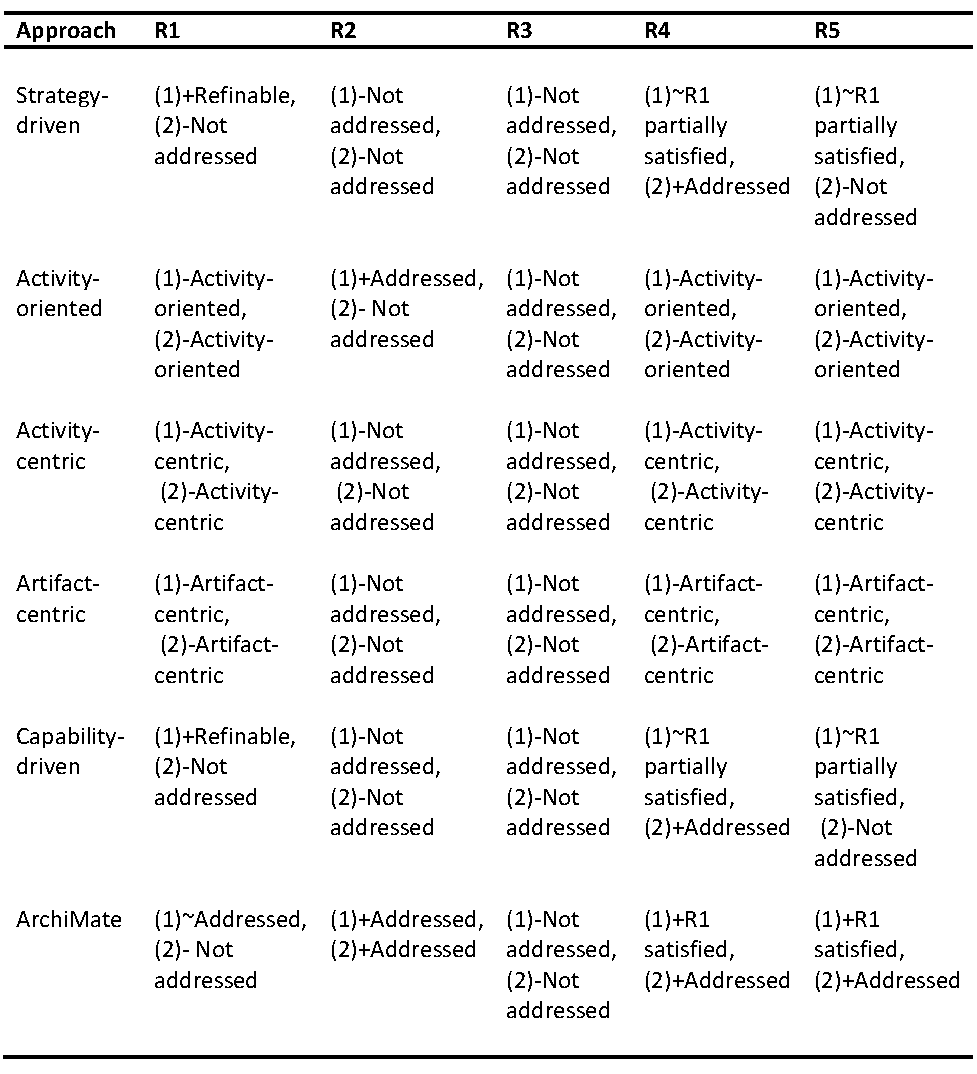
\includegraphics[width= \textwidth]{Approach.pdf}
 	\caption{Summary of the Evaluation}
 	\label{tab:evaluationoftheapproach}
 \end{table} 


